\chapter{Brazil Nut Effect (BNE)}
\label{chap:BNE}
    Historically, the phenomenon known as BNE was identified in Brazil nut exports, which were taken in containers on ships leaving Brazil, and whenever they arrived at their destination, it was observed that the largest nuts were at the top. Initially it was thought that Brazilian traders arranged the nuts so that the largest were on top and the smaller and broken ones at the bottom. After investigation, it was verified that the larger nuts rise due to the vibration that the containers suffered during transport \cite{Caio-Tese}. 

    The BNE occurs when grains of different sizes segregate, causing larger grains segregate from smaller ones. The segregation effect can be seen when a system is shaken, or a shear cycle is imposed \cite{Granular_Physics}. This phenomenon is associated with the granular phase of the system. In a solid-like granular system, the larger grain is static. With agitation, the system changes to a liquid state, allowing the movement of grains in the system \cite{Why_the_Brazil_nuts_are_on_top}. The movement of the material occurs in convection currents that form close to the walls, or with the ratchet effect \cite{Effects_of_convection_and_friction_on_size_segregation_in_vibrated_granular_beds, Scaling_behavior_in_convection-driven_Brazil-nut_effect, Inertia_in_the_Brazil_nut_problem, The_water-enhance_Brazil_nut_effect}, both cases allow small grains fill the space previously occupied by the larger grain, rising the larger grain. Figure \ref{fig:BNE_hejmady_convection} shows the evolution of the convection currents in a confined media. Once smaller grains collectively move to fill the void left by larger grains, smaller grains imped their downward motion; these correlations are at the basis of the observed size segregation. The ratchet effect is the granular solid-like behavior in below larger grains and the granular liquid-like behavior, where larger grains can move. The ratchet effect is also related to the Reynolds dilatancy, since the stress increases and the granular configuration changes.

\begin{figure}
    \centering
    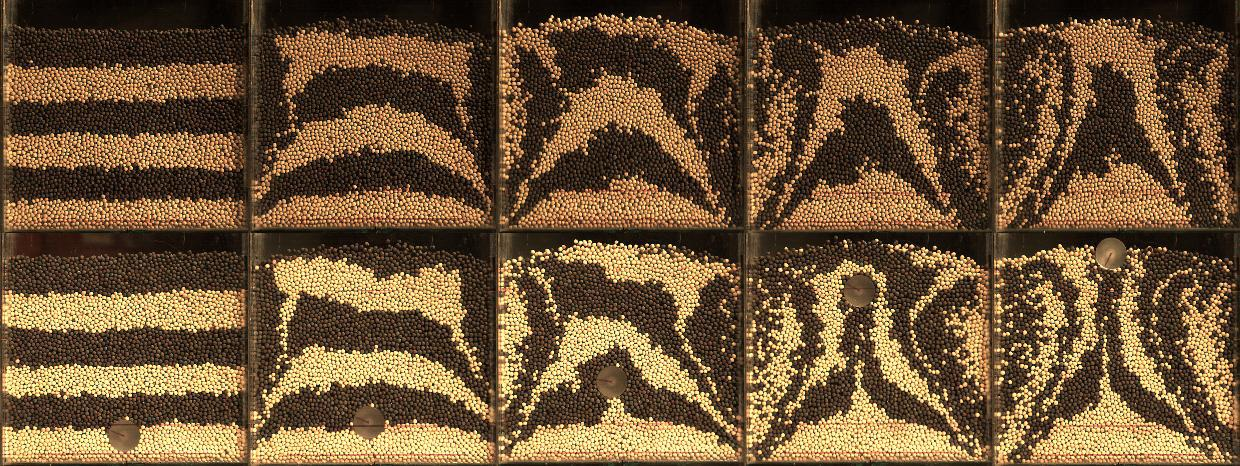
\includegraphics[width=0.65\textwidth]{04-figuras/BNE_Hejmady_Convection.png}
    \caption[Granular convection in vibrated bed.]{Evolution of the vibrated bed. Top Panels are without intruder, while bottom Panels are with an intruder. Black and yellow layers are made of mustard grains. Figure taken from \cite{Scaling_behavior_in_convection-driven_Brazil-nut_effect}.}
    \label{fig:BNE_hejmady_convection}
\end{figure}

    One of the firsts attempts to explain the BNE was made by Rosato \textit{et al.} \cite{Why_the_Brazil_nuts_are_on_top} using Monte Carlo simulations and inspired many works to classify the roles of the parameters. As an example of the larger grain rising with respect to time, Figure \ref{fig:BNE_rosato}.

\begin{figure}
    \centering
    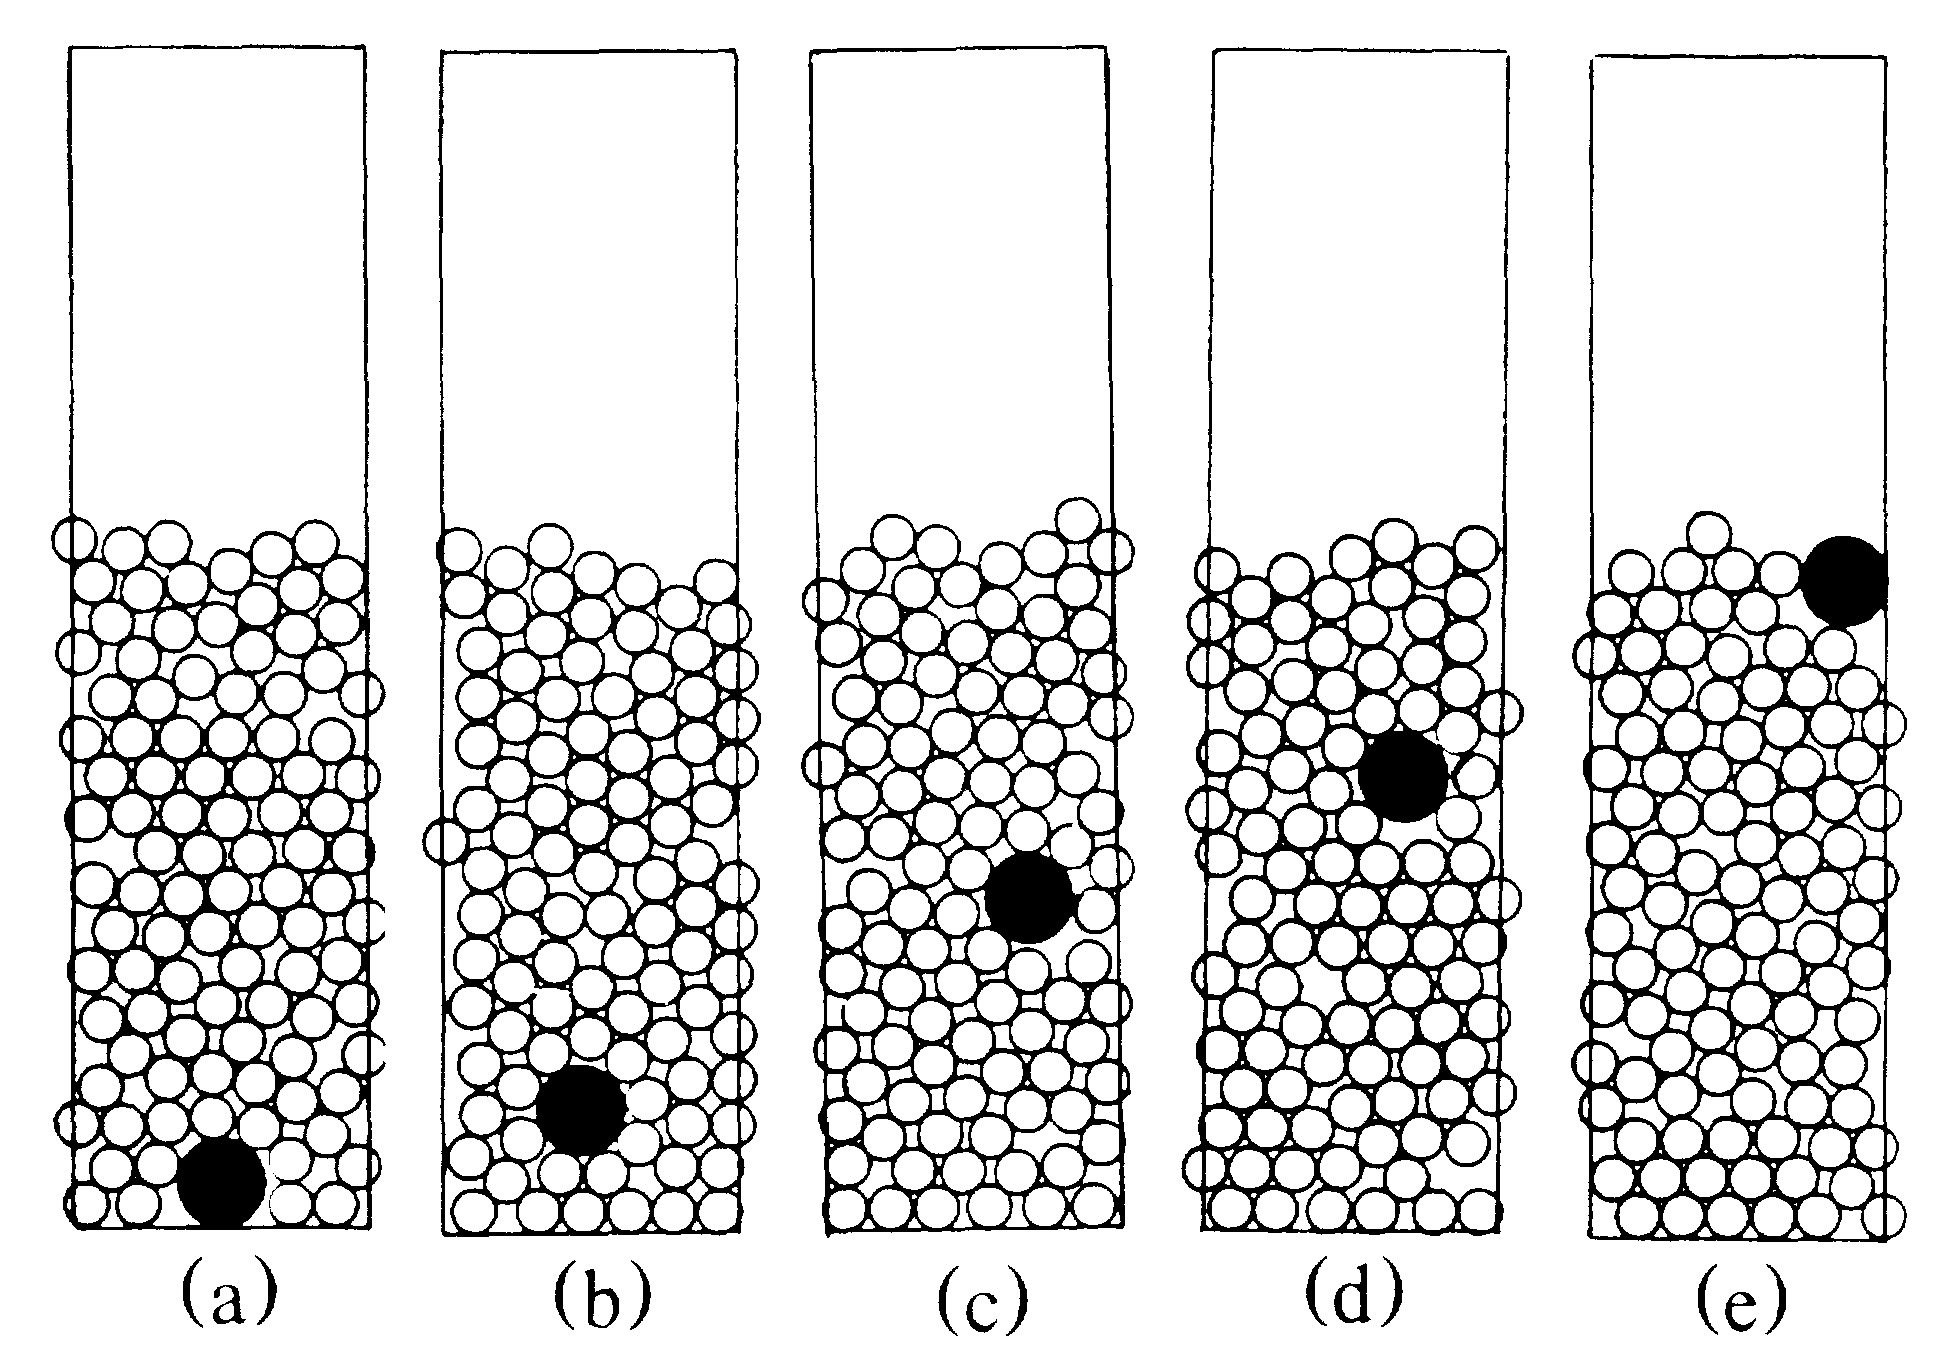
\includegraphics[width=0.65\textwidth]{04-figuras/BNE_Rosato.png}
    \caption[BNE cycles.]{Temporal evolution of shaken system of particles with periodic boundary conditions using Monte Carlo simulation. Initial configuration in Panel (a) and equally time spaced from Panels (a) to (e). Figure taken from \cite{Why_the_Brazil_nuts_are_on_top}.}
    \label{fig:BNE_rosato}
\end{figure}

    The most important number used in the BNE studies is the dimensionless acceleration, shown in the equation \ref{equ:gamma}. The dimensionless number is a comparison between the maximum amplitude of the vibrational acceleration and gravity. 
\begin{equation}
    \label{equ:gamma}
    \Gamma = \frac{A\omega^{2}}{g},
\end{equation}
where $\Gamma$ a dimensionless number that compares shaken acceleration with gravity, $A$ is the system amplitude of the vibration, $\omega$ is the frequency of vibration, and $g$ is the value of gravity. When $\Gamma > $ 1, then the intruder can rise, since the ascending part of the oscillation rises the magnitude of the chain forces in the media, but when the system is descending the lighter grains occupies the void space left by the bead, causing the ratchet effect. If $\Gamma < $ 1, then the intruder is not able to move, since chain forces stays there. This is the basic explanation, but not all cases work like it, as we see in some of our simulations, in Chapter \ref{chap:Resultados-BNE}.

    An experimental problem is proposed in \cite{Inertia_in_the_Brazil_nut_problem}, like we study in Chapter \ref{chap:Resultados-BNE}. In their experiment a metallic bead is placed at bottom and then agitated. They use a cylinder silo and spherical grains with size ratio between intruder and media of 3, and $\Gamma$ varies from 2.6 to 3.4, which leads the bead to rise over the media. There is a collapse of the curves involving the intruder position, the amplitude of the vibration $A$ and the oscillation period $\omega$ like in figure \ref{fig:BNE_molinari}. What we could find in our simulations is that frictionless walls also cause the bead to rise through convection currents, and the ascent ratio is similar with and without friction on the walls, see Figure \ref{fig:BNE25000_sem_Atrito_Parede}.

\begin{figure}
    \centering
    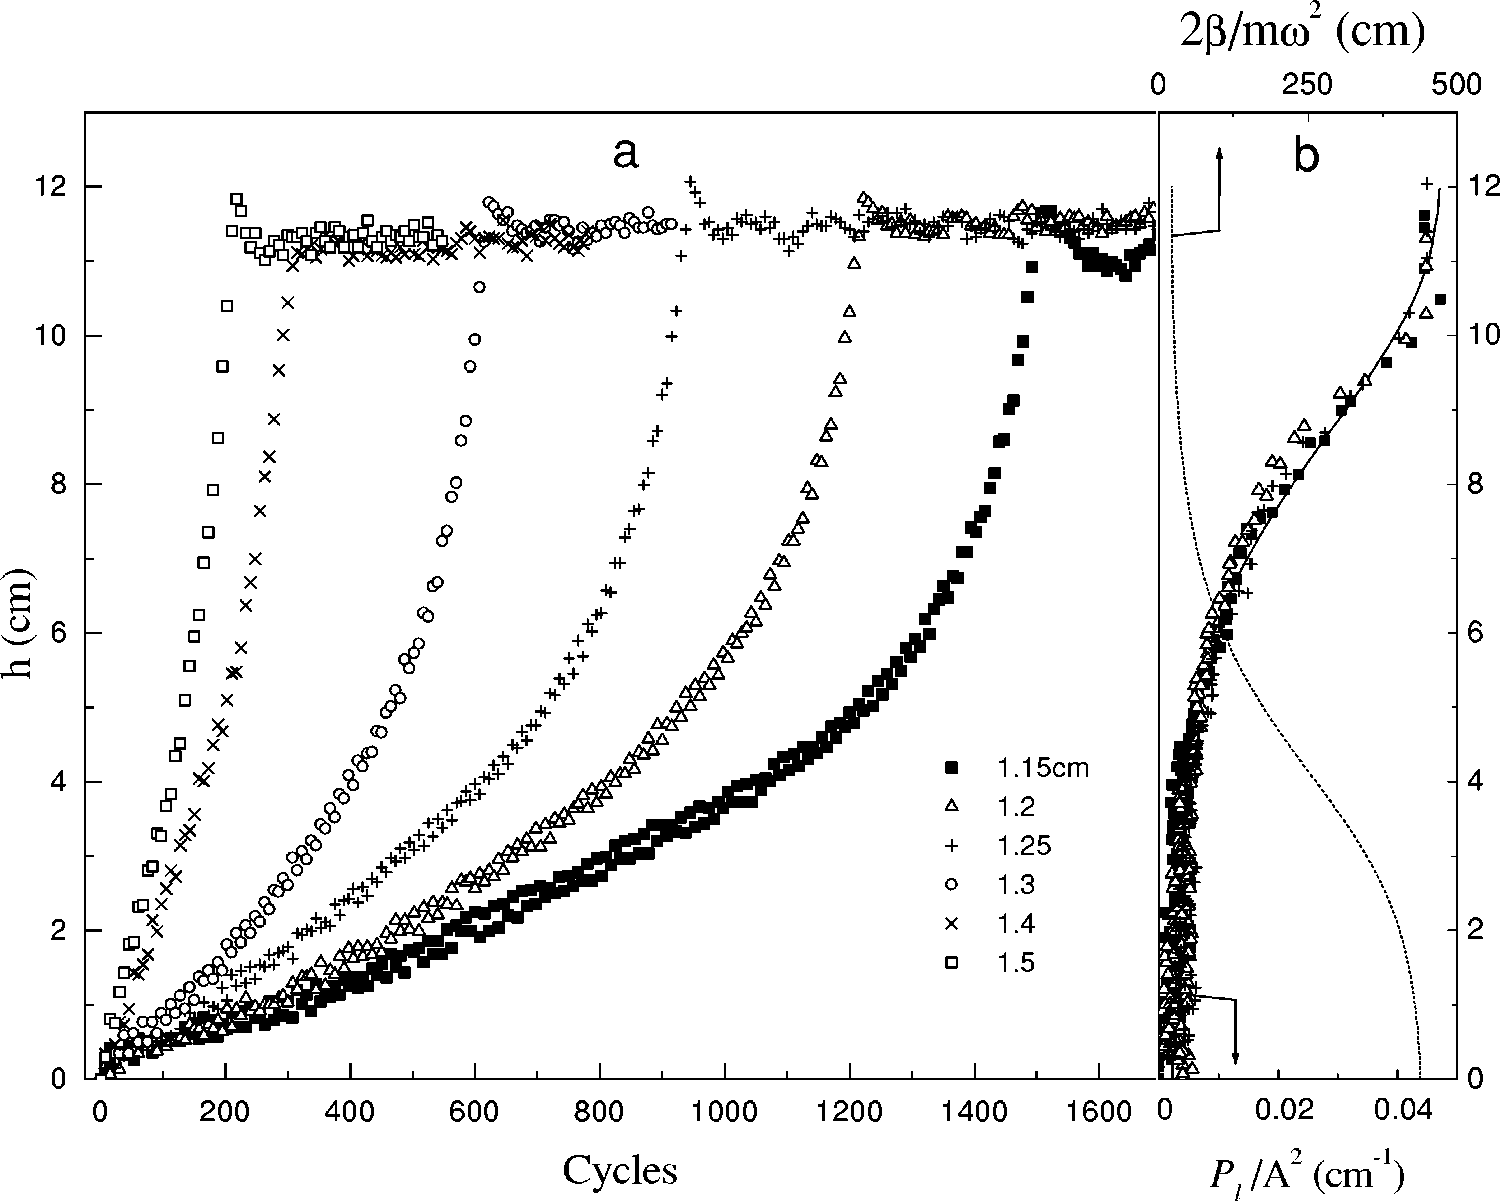
\includegraphics[width=0.65\textwidth]{04-figuras/BNE_Molinari.png}
    \caption[Intruder height in an agitated media.]{Evolution of the bead in an agitated media within a cylinder silo. Panel (a) shows the height of the intruder versus time, while Panel (b) shows the collapse of the curves. Figure taken from \cite{Inertia_in_the_Brazil_nut_problem}.}
    \label{fig:BNE_molinari}
\end{figure}

    The BNE is also influenced by the fluid that surrounds the media. In some cases, the air is relevant in the convection currents, and then leading to segregation, while vacuum leads to mixing \cite{Brazil-Nut_effect_Size_separation_of_granular_particles, Inertia_in_the_Brazil_nut_problem}. A more viscous fluid than air, like water, changes the regime of ascension of the bead, and the main mechanism that explains it is not the drag it self but the enhance of the ratcheting effect \cite{The_water-enhance_Brazil_nut_effect}.

    Several phase diagrams were observed for some of the BNE parameters. The two main variables usually analysed are the ratio of the diameters of grains and the ratio of densities of grains, as shown in Figure \ref{fig:BNE_mobius}. Another BNE phase diagram proposed by \cite{Scaling_behavior_in_convection-driven_Brazil-nut_effect} takes into account the dimensionless acceleration $\Gamma$ and the vibration threshold velocity $v_c = A \omega$.

\begin{figure}
    \centering
    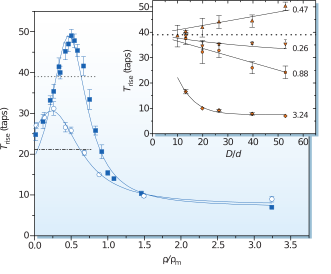
\includegraphics[width=0.65\textwidth]{04-figuras/BNE_Mobius.png}
    \caption[Phase diagram of BNE: density ratio and size ratio.]{BNE dependence on density and size ratio. The ascent time $T_{rise}$ in the main Panel versus density rate, with size ratio of 5.08 between intruder and grains with different atmospheric pressures: 1 atm. in squares ($\textcolor{blue}{\blacksquare}$) and 90 torr in circles ($\textcolor{blue}{\circ}$). The ascent time $T_{rise}$ versus the size ratio for different density ratios: 0.44, 0.48, 0.88 and 3.1. Figure taken from \cite{Brazil-Nut_effect_Size_separation_of_granular_particles}.}
    \label{fig:BNE_mobius}
\end{figure}

\begin{figure}
    \centering
    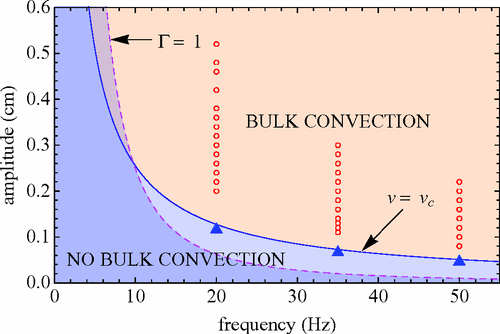
\includegraphics[width=0.65\textwidth]{04-figuras/BNE_Hejmady_PhaseSpace.png}
    \caption[Phase diagram of BNE: $\Gamma$ and $v_c$.]{BNE dependence on the dimensionless acceleration $\Gamma$ and a critical velocity $v_c$. Values of $\Gamma$ < 1 makes the intruder not rise, but also a $v < A \omega$. Figure taken from \cite{Scaling_behavior_in_convection-driven_Brazil-nut_effect}.}
    \label{fig:BNE_hejmady_convection}
\end{figure}

    Another correlated phenomena to BNE is the Reverse BNE (RBNE), in which the bead instead of rises it sinks. Many works enhanced the characterization of BNE and RBNE, in theoretical field, experimental results and numerical simulations \cite{A_Horizontal_Brazil-Nut_Effect_and_Its_Reverse, Brazil-nut_effect_versus_reverse_Brazil-nut_effect_in_a_moderately_dense_granular_fluid, Categorization_of_Brazil_nut_and_its_reverse_under_less-convective_conditions_for_microgravity_geology, Competition_of_Brazil_nut_effect_buoyancy_and_inelasticity_induced_segregation_in_a_granular_mixture, Reverse_Brazil_Nut_Problem_Competition_between_Percolation_and_Condensation, Reverse_buoyancy_in_a_vibrated_granular_bed_Computer_Simulations, Reversing_the_Brazil-Nut_Effect_Competition_between_Percolation_and_Condensation, Segregation_in_a_fluidized_binary_granular_mixture_Competition_between_buoyancy_and_geometric_forces, Simple_model_for_reverse_buoyancy_in_a_vibrated_granular_system, Hydrodynamic_theory_for_reverse_brazil_nut_segregation_and_the_non-monotonic_ascension_dynamics}. Some of these diagrams are presented here in Figures \ref{fig:RBNE_breu}, \ref{fig:RBNE_schnautz} and \ref{fig:RBNE_trujillo}.

\begin{figure}
    \centering
    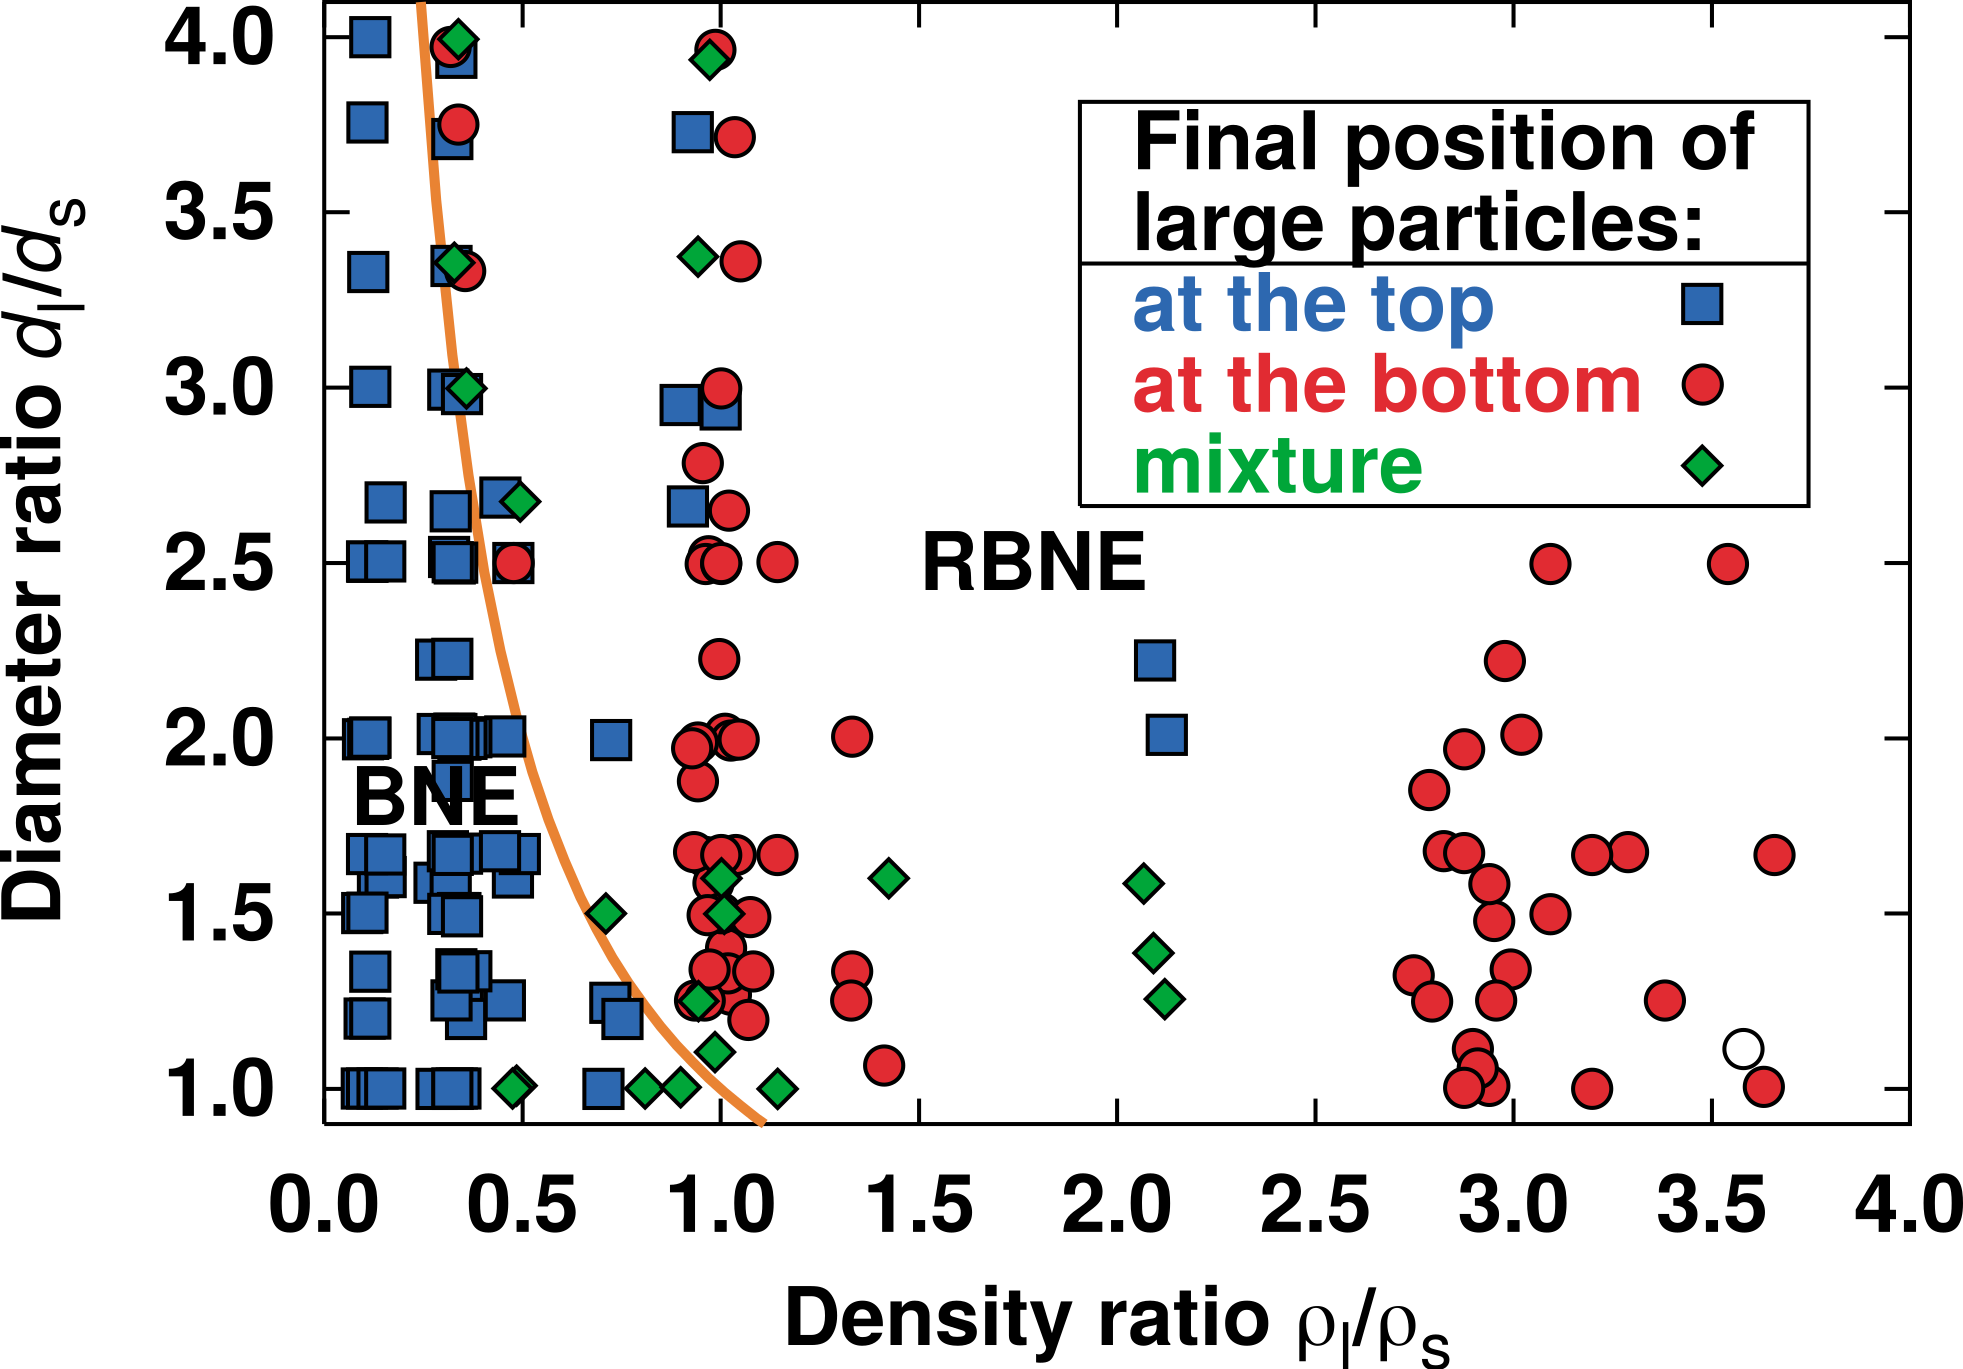
\includegraphics[width=0.65\textwidth]{04-figuras/BNE_Breu.png}
    \caption[Phase diagram of BNE/RBNE from experiment: density ratio and size ratio.]{BNE and RBNE dependence on the density ratio and the size ratio in vibrated base. The diagram shows the regime where beads rises in blue ($\textcolor{blue}{\blacksquare}$) causing the BNE, sinks in red ($\textcolor{red}{\blacksquare}$) and is mixed in green ($\textcolor{green}{\blacksquare}$). Figure taken from \cite{Reversing_the_Brazil-Nut_Effect_Competition_between_Percolation_and_Condensation}.}
    \label{fig:RBNE_breu}
\end{figure}

\begin{figure}
    \centering
    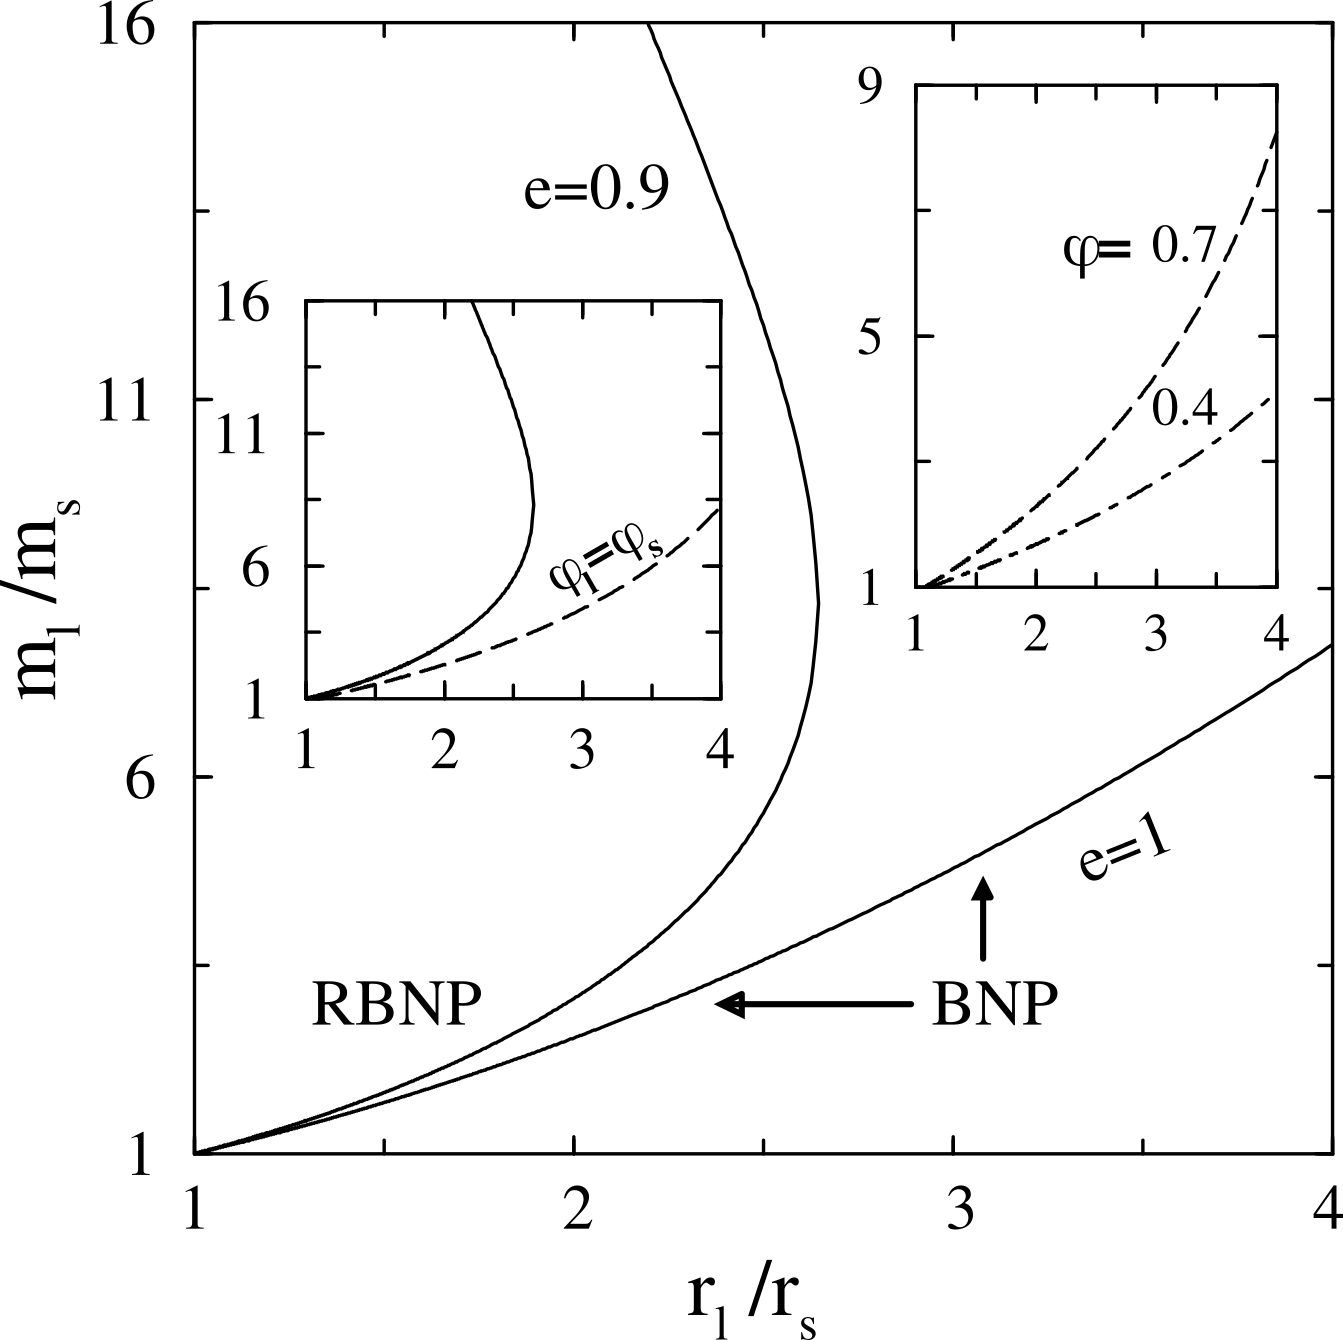
\includegraphics[width=0.65\textwidth]{04-figuras/BNE_Trujillo.png}
    \caption[Phase diagram of BNE/RBNE from analytics: density ratio and size ratio.]{BNE and RBNE dependence on the density ratio and the size ratio in vibrated base. The diagram shows the BNE-RBNE regime extracted from analytical equations of the forces in the system. $e$ is the restitution coefficient, $\phi$ is the packing fraction, $\phi_{l}$ is the portion of the packing fraction related to the intruders, $\phi_{s}$ is the packing fraction of the other grains. Left inset: phase diagram with $e$ = 0.9, $\phi_{l} / \phi_{s}$ = 10$^{-8}$ (solid curve) and $\phi_{l} / \phi_{s}$ = 1 (dashed curve). Right inset: phase diagram with $e$ = 0.9, $\phi_{l} / \phi_{s}$ = 1, $\phi$ = 0.7 (dashed curve) and $\phi$ = 0.4 (dot-dashed curve). Figure taken from \cite{Segregation_in_a_fluidized_binary_granular_mixture_Competition_between_buoyancy_and_geometric_forces}.}
    \label{fig:RBNE_trujillo}
\end{figure}

\begin{figure}
    \centering
    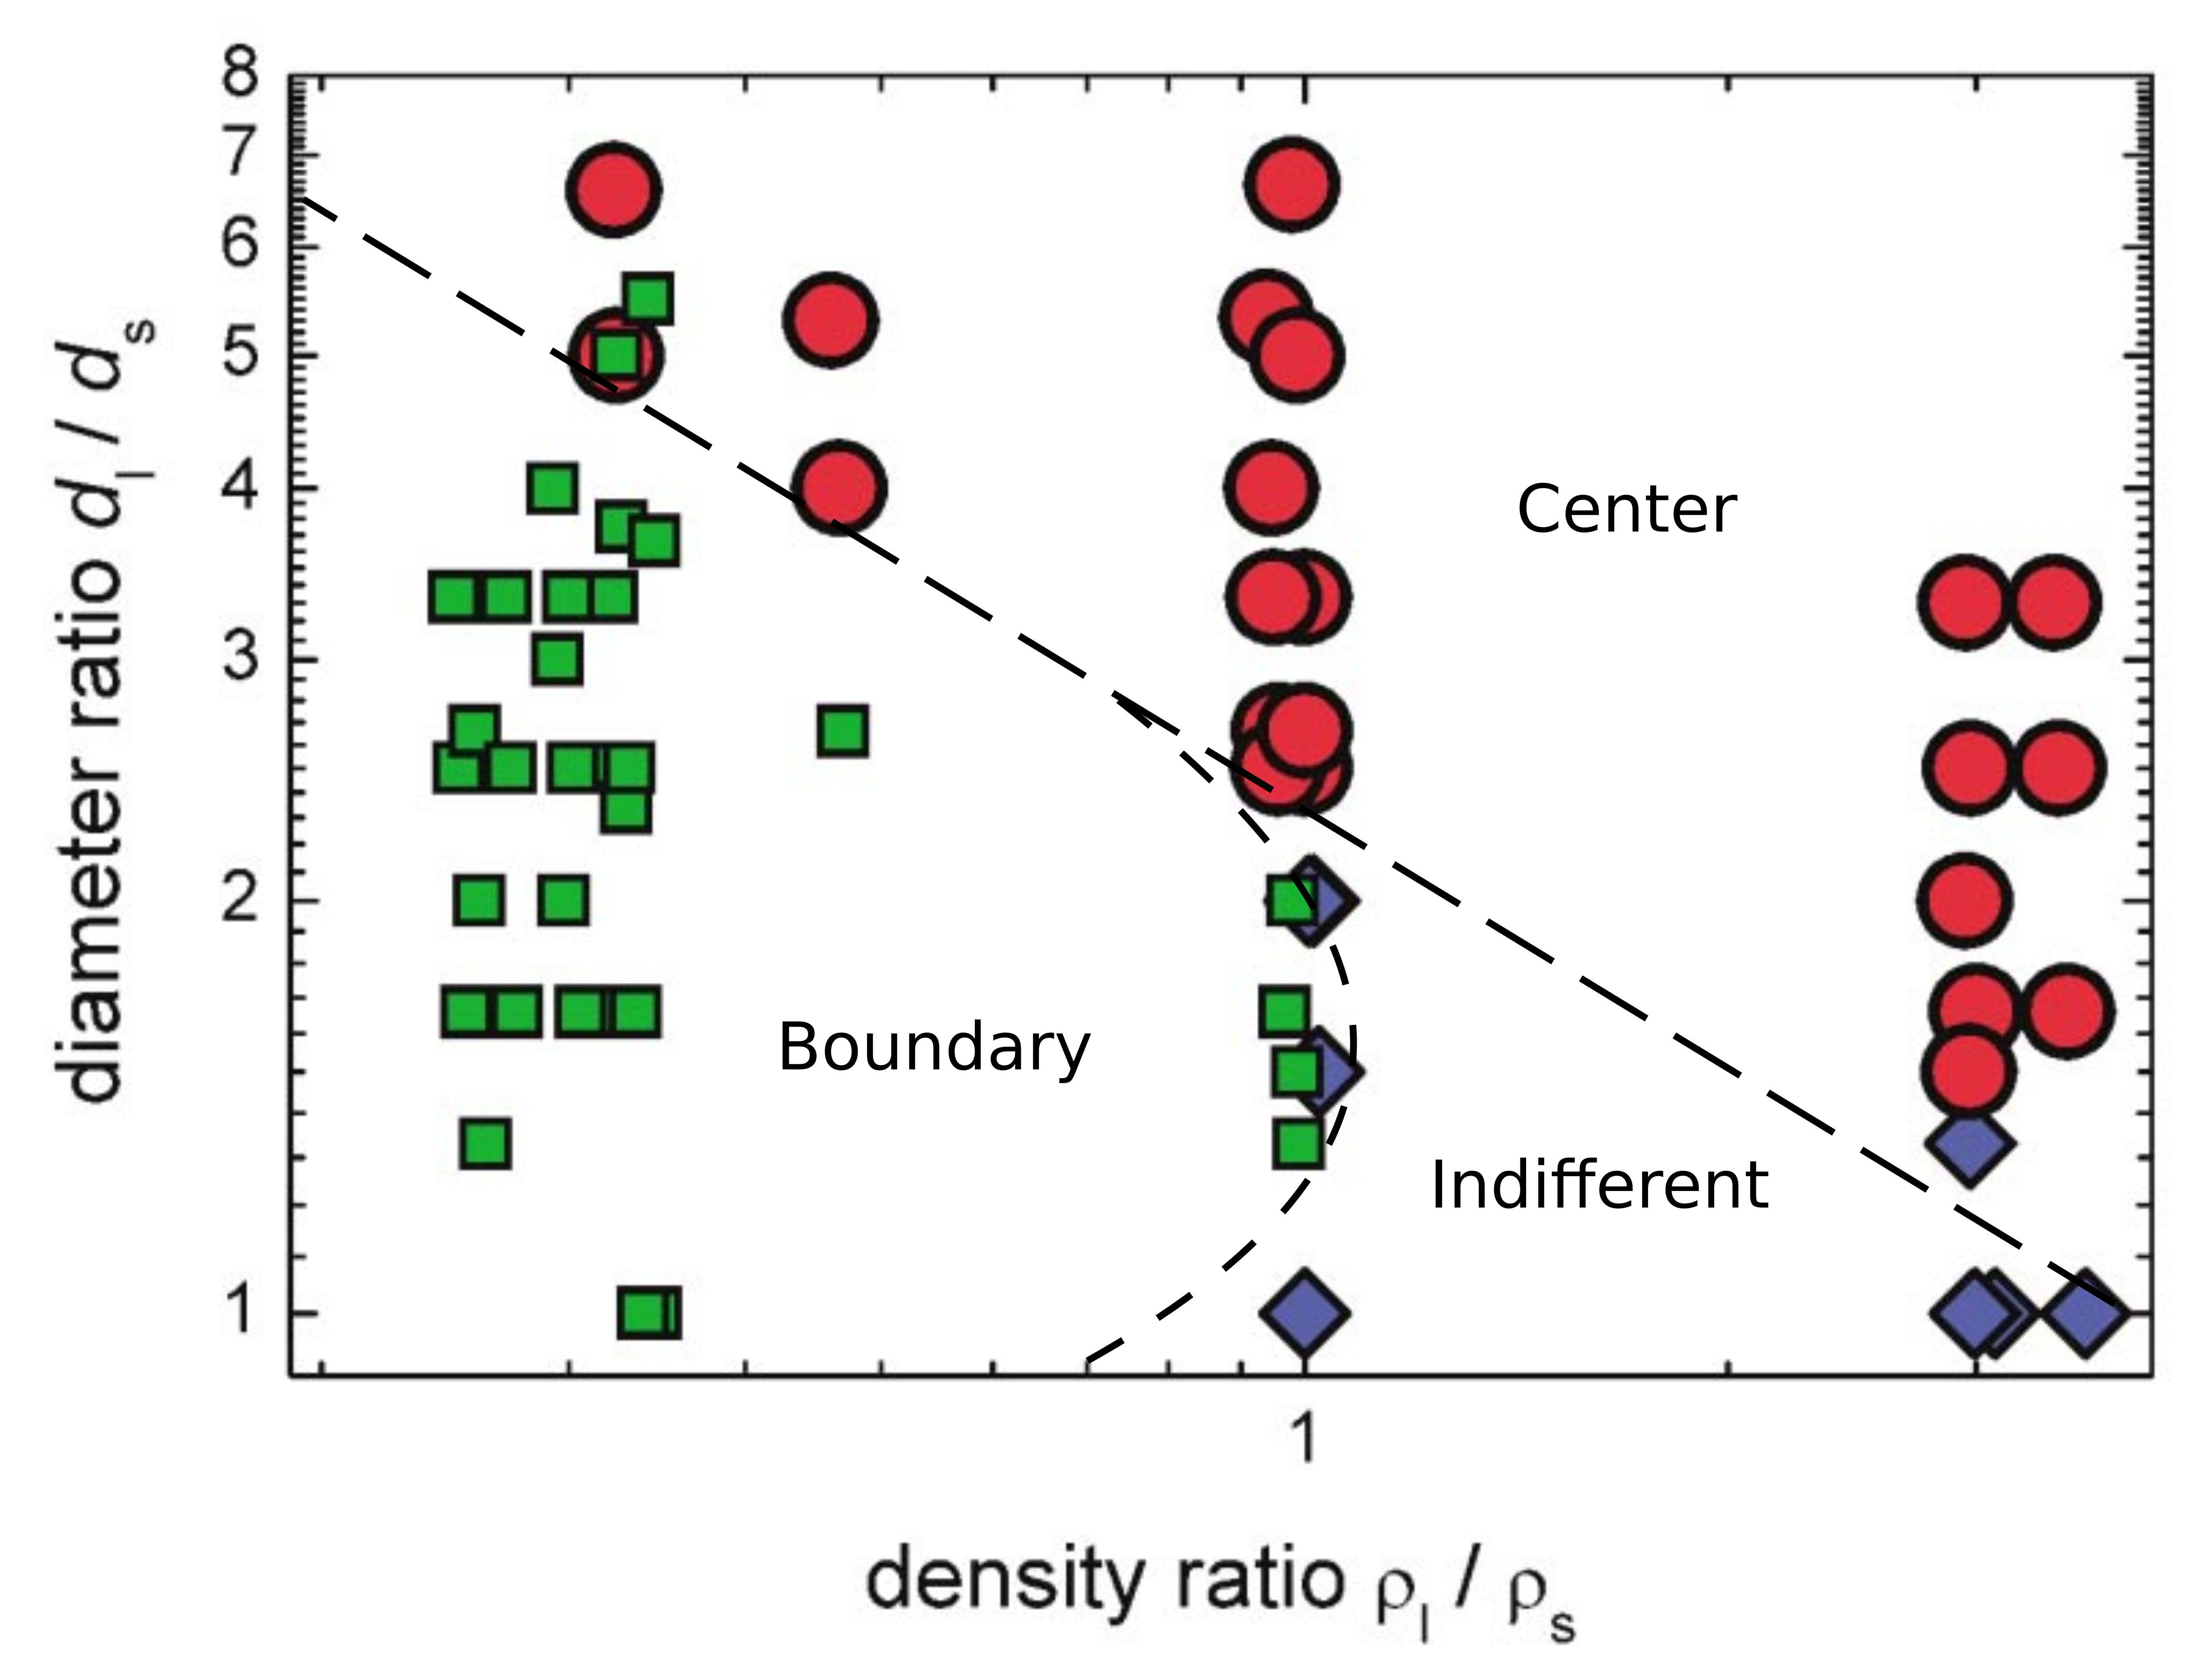
\includegraphics[width=0.65\textwidth]{04-figuras/BNE_Schnautz.png}
    \caption[Phase diagram of BNE/RBNE in swirling: density ratio and size ratio.]{BNE and RBNE dependence on the density ratio and the size ratio in swirling base. The diagram shows the regime where beads segregates in red ($\textcolor{red}{\CIRCLE}$), aggregates in green ($\textcolor{green}{\blacksquare}$) and is indifferent in blue ($\textcolor{blue}{\Diamondblack}$). Figure taken from \cite{A_Horizontal_Brazil-Nut_Effect_and_Its_Reverse}.}
    \label{fig:RBNE_schnautz}
\end{figure}

    Recently the Reference \cite{Size_segregation_of_irregular_granular_materials_captured_by_time-resolved_3D_imaging} experimentally shows that in a mixture of irregular ellipsoidal shape firstly reorient vertically, but without changing significantly their height; secondly, the grains rise upwards, and while doing so, they still tend to stay vertically aligned; and finally, when the grains reach the top, they tend to realign horizontally on the surface.

    If the intruder of the media has a non uniform distribution geometry, like a polar particle, inserted in a layer of circular grains, and when the media is agitated, the intruder starts to "self-propel" at the direction it is oriented \cite{Symmetry_properties_of_the_large-deviation_function_of_the_velocity_of_a_self-propelled_polar_particle}. This is another property that non uniform shaken granular exhibit, reorienting the position or "propelling-itself".

%Reverse BNE: A_Horizontal_Brazil-Nut_Effect_and_Its_Reverse, Brazil-nut_effect_versus_reverse_Brazil-nut_effect_in_a_moderately_dense_granular_fluid, Caracterization_of_Brazil_nut_and_its_reverse_under_less-convective_conditions_for_microgravity_geology, Competition_of_Brazil_nut_effect_buoyancy_and_inelasticity_induced_segregation_in_a_granular_mixture, Reverse_Brazil_Nut_Problem_Competition_between_Percolation_and_Condensation, Reverse_buoyancy_in_a_vibrated_granular_bed_Computer_Simulations, Reversing_the_Brazil-Nut_Effect_Competition_between_Percolation_and_Condensation, Segregation_in_a_fluidized_binary_granular_mixture_Competition_between_buoyancy_and_geometric_forces, Simple_model_for_reverse_buoyancy_in_a_vibrated_granular_system, Hydrodynamic theory for reverse brazil nut segregation and the non-monotonic ascension dynamics
%Vibrações verticais: Inertia_in_the_Brazil_nut_problem, The_water-enhance_Brazil_nut_effect, Brazil-Nut_effect_Size_separation_of_granular_particles, Caracterization_of_Brazil_nut_and_its_reverse_under_less-convective_conditions_for_microgravity_geology, Competition_of_Brazil_nut_effect_buoyancy_and_inelasticity_induced_segregation_in_a_granular_mixture, Reverse_buoyancy_in_a_vibrated_granular_bed_Computer_Simulations, Reversing_the_Brazil-Nut_Effect_Competition_between_Percolation_and_Condensation, Scaling_behavior_in_convection-driven_Brazil-nut_effect
%Vibrações laterais: Size_segregation_of_irregular_granular_materials_captured_by_time-resolved_3D_imaging, A_Horizontal_Brazil-Nut_Effect_and_Its_Reverse, 

    Next Chapter, we describe the results of our BNE simulations using the techniques presented in Chapter \ref{chap:DEM}.

%    Inertia_in_the_Brazil_nut_problem -> Atribui a convecção ao atrito das paredes e colapsa as curvas de ascensão.
%    The_water-enhance_Brazil_nut_effect -> Uso do fluido intersticial com BNE.
%    Why_the_Brazil_Nuts_are_on_top -> Atribui o BNE ao efeito catraca, usando Monte Carlo e desprezando atrito e a massa é desprezível para o efeito.
%    A_Horizontal_Brazil-Nut_Effect_and_Its_Reverse -> Vibra horizontalmente e com diferentes materiais (densidades), reproduz BNE (ida para o centro) e rBNE (ida para as bordas). Frequências de 0.5 à 2Hz, amplitude de $3,175n$mm, com $n$ variando de $3 ... 7$, diâmetro médio dos grãos de 6mm, diâmetro do intruso $1,3 ... 7$ vezes o diâmetro dos grãos e coeficiente de atrito de $0,67$. Exibe um diagrama de fase Diâmetro/Densidade.
%    Brazil-Nut_effect_Size_separation_of_granular_particles -> Descreve o fenômeno em função do diâmetro e da densidade, fixa a frequência em $13$Hz e a amplitude em $7,35$mm e o diâmetro do grão menor em $0,5$mm, ou seja, a relação amplitude e diâmetro do grão é de $14,7$ vezes. Diâmetro do intruso pode chegar à $25,4$mm, o equivalente $50800$ vezes o diâmetro do grão.
%    Brazil-nut_effect_versus_reverse_Brazil-nut_effect_in_a_moderately_dense_granular_fluid -> Analítico/teórico sobre os planos de fase das regiões BNE e rBNE em função do diagrama Diâmetro/Densidade com coeficiente de compactação e restituição.
%    Caracterization_of_Brazil_nut_and_its_reverse_under_less-convective_conditions_for_microgravity_geology -> Reproduz o BNE em condição fechada, porém com atrito baixo entre parede/grão, com condições de aceleração menores q a gravidade.
%    Competition_of_Brazil_nut_effect_buoyancy_and_inelasticity_induced_segregation_in_a_granular_mixture -> Compara os resultados do BNE em função das massas, diâmetros e coeficientes de restituição.
%    Reverse_Brazil_Nut_Problem_Competition_between_Percolation_and_Condensation -> Mostra o diagrama qualitativo da transição BNE para rBNE em função da razão dos diâmetros pelas massas. Relaciona a temperatura granular.
%    Reverse_buoyancy_in_a_vibrated_granular_bed_Computer_Simulations -> Insere um fluido como amortizador e demonstra as forças e seus efeitos.
%    Reversing_the_Brazil-Nut_Effect_Competition_between_Percolation_and_Condensation -> Mostra o diagrama BNE/rBNE em função da densidade versus diâmetro, com o diagrama de frequência por aceleração normalizada.
%    Scaling_behavior_in_convection-driven_Brazil-nut_effect ->  mostra o esquema de convecção para a contribuição no BNE
%    Segregation_in_a_fluidized_binary_granular_mixture_Competition_between_buoyancy_and_geometric_forces -> Diagrama BNE/rBNE densidade versus diâmetro
%    Simple_model_for_reverse_buoyancy_in_a_vibrated_granular_system -> Velocidade no BNE/rBNE densidade
%    Study_the_effect_of_vibration_frequency_and_amplitude_on_the_quality_of_fluidization_of_a_vibrated_granular_flow_using_discrete_element_method -> Caracteriza o fluido em função da altura do sistema.

%    Size_separation_in_vibrated_granular_matter -> Compilado dos artigos acima

%    Convection_Cells_in_Vibrating_Granular_Media -> Em relação ao BNE não é mostrado, uma vez q a distribuição dos raios dos grãos são próximas entre si. Mostra a convecção na agitação dos granulares, mesmo quando possuem condição periódica de contorno. Porém a agitação é muito alta.
